\documentclass{article}


\usepackage[utf8]{inputenc}
\usepackage{amsmath}
\usepackage{amsfonts}
\usepackage{amssymb}
\usepackage{amsthm}
\usepackage[margin=1in]{geometry} % for smaller margins

% for figures
\usepackage{graphicx}
\graphicspath{ {.} }

% Theorem environments
\theoremstyle{remark}
\newtheorem{remark}{Remark}
\newtheorem{thm}{Theorem}
\newtheorem{lemma}{Lemma}
\newtheorem{prop}{Proposition}
\newtheorem{defn}{Definition}
\newtheorem{exa}{Example}

% commands
\newcommand{\e}{ \varepsilon }
\newcommand{\R}{ \mathbb{R} }
\newcommand{\Z}{ \mathbb{Z} }
\newcommand{\D}{ \partial }
\renewcommand{\S}{ \mathbb{S} }
\renewcommand{\L}{ \mathbb{L} }
\newcommand{\halfspace}{ \mathbb{H} }
\newcommand{\sphere}{ \mathbb{S} }
\newcommand{\eL}{ \mathbb{L} } % RRS notation
\newcommand{\fancy}{ \mathcal }
\newcommand{\tr}{ \text{tr} }
\newcommand{\norm}[1]{\left\lVert#1\right\rVert}
\newcommand{\supp}{\text{supp}}
\newcommand{\proj}{\text{proj}}
\newcommand{\spa}{\text{span}}
\newcommand{\rk}{\text{rk}}
\newcommand{\diam}{\text{diam}}



\title{HW3: 1d energy balance model}

\begin{document}

\maketitle
Link to github repository: 


Let $T_0$ be an initial (meridionally-averaged) temperature distribution, set to be 
$T_0(x) = 10^\circ C$ for all $x \in [0,1]$, the meridional coordinate. We assume that
the temperature $T(t,x)$ of the system evolves according to
\begin{align}
	\D_t T & = QS(x)a(x) - (A+BT) + \mathbb{D}[T]	\label{heat_eq} \\
	\text{subject to } T(t,x)\Big|_{t=0} & = T_0		\label{ic}		\\
	(1-x^2)\frac{\D T}{\D x}(t,x)\Big|_{x=0,1} & = 0	\label{noflux}.
\end{align}
where $Q$ is the solar constant, $S(x)$ the solar radiation distribution, and $a(x)$
the co-albedo; together they comprise a term modelling the incoming energy radiated from the sun. 
The term which representing the outgoing radiation from earth,
modeled by the Stefan-Boltzmann law, is linearized as $\sigma T^4 \sim (A+BT)$ for some 
parameters $A$ and $B$. In atmospheric temperature ranges like $[-10,40]^\circ C$,
this linearization is a good approximation. Furthermore, the diffusion operator $\mathbb{D}$
takes the form
\begin{align}
	\mathbb{D}[f](x) \doteq D\frac{\D}{\D x}\left( (1-x^2) \frac{\D f}{dx} \right).
\end{align}
for some positive parameter $D$, the diffusion coefficient.
% More general elliptic operators also considered in North et al 81. What about boundary
% conditions for these? See also: Fuchs theorem, Stakgold, Gilbarg-Trudinger.
% ALSO:
% should the same (co-)albedo coefficient be used in \sigma T^4 term, for 'earth as
% gray body' approximation? TODO
To this second-order differential operator with boundary conditions \eqref{noflux}, 
we might consider the associated eigenvalue problem
\begin{align}\label{eigenvalue_prob}
	\mathbb{D}[f](x) = -\lambda f(x).
\end{align}

Note that we have taken the following special forms for the solar radiation and albedo
terms:
\begin{align}
	S(x) & = S_0 + S_2 P_2(x)	\\
	a(x) & = a_0 + a_2 P_2(x)
\end{align}
subject to the constraint
\begin{align}
	\int_0^1 S(x) = 1.
\end{align}
% What accounts for this solar irradiance difference across x--solely effect of different 
% distance measurements?
We think of $S$ as a distribution of solar irradiance over the meridional coordinate. The
co-albedo coefficient $a(x)$ likewise has some spatial dependence. In this way,
with $QS(x)a(x)$ the average power per meter squared, the power density at $x$ is modulated 
by the distributions of solar irradiance as well as the co-albedo. 
The net difference between these effects forces the heat equation above.
Plots of both as a function of $\sin(\theta)$ with $\theta \in [0,\frac{\pi}{2}]$ are below.

\begin{figure}
\centering
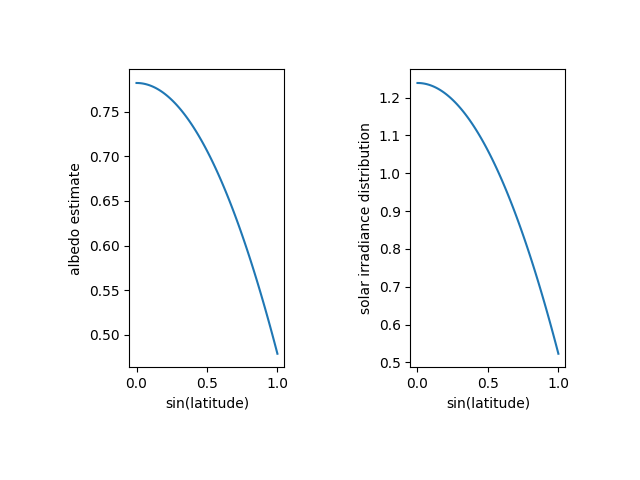
\includegraphics{albedo_irradiance.png}
\end{figure}

\subsection{1d heat equation with ODEINT}

Here we describe some of the code \verb+in energy_bal1d.py+. In particular,
we focus on the diffusion operator, in which the boundary conditions of the
model are encoded. At the equator grid-point, $i=0$, we use the boundary 
condition to rewrite diffusion operator. We invoke a GHOST POINT at $i=-1$, 
where the no-flux condition, implemented via a leapfrog difference, is enforced:
\begin{align}
	\frac{\D T}{\D x}\Big|_{x=0} \sim D_h^{leap}[T][0] 
	\doteq 1/(2h)(T[1]-T[-1]) = 0.
\end{align}
Therefore, this boundary condition introduces the constraint 
$T[0] = T[2]$. We may then use to re-write the only non-degenerate
portion of the discretized diffusion operator $\mathbb{D}_h[T]$ at $i=0$, i.e., 
the second-order term of the central-difference operator approximating
the term $\frac{\D^2 T}{\D x^2}$:
\begin{align}
	\mathbb{D}_h[T][0] = D(T[1] - 2T[0] + T[-1])/(h^2)	
				= 2D(T[1] - T[0])/(h^2)
\end{align}

At the pole, since $x[N] = 1$ here, the only non-degenerate part of the diffusion operator
is the first-order term:
\begin{align}
	\frac{\D T}{\D x}(t,1) = (1-1^2)\frac{\D^2 T(t,1)}{\D x^2} - 2 \frac{\D T(t,1)}{\D x}
			= -2 \frac{\D T(1)}{\D x}
\end{align}
which is implemented via a one-sided difference of $O(h)$ accuracy. The interior updates 
are discretized by a combination of a central-difference scheme for the second-order term
and a leap-frog difference scheme for the first-order term.

A plot of the solution found with ODEINT is included below, using a grid resolution of 
$n = 100$, over a time period of 30 years with monthly time steps:

\begin{figure}
\centering
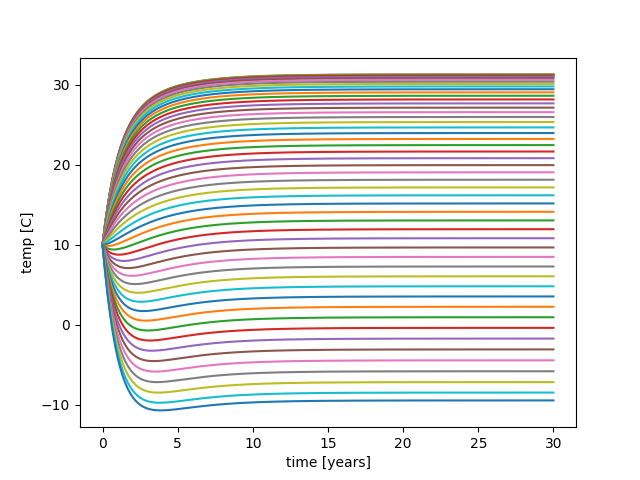
\includegraphics{odeint_profile.png}
\end{figure}

We want to benchmark this solution against the analytic solution. The code for this is in
\verb+analytic_benchmarking.py+. This is described in the third section.



\subsection{Implicit euler scheme}

% 'method of lines' according to Leveque
Discretizing first in space, we consider the first-order (in time) ODE 
\begin{align}\label{methodoflines}
	\frac{d}{dt} T(t,x[i]) = QS(x[i])a(x[i]) - (A+BT)(x[i]) + \mathbb{D}_h[T]_i(x).
\end{align}
We now have, for each grid point $x[i]$, $i = 0, \ldots N$ an ODE to solve given
initial condition $T_0(x[i]) = 10$. We discretize this according to the implicit
Euler, for the stability properties of its solutions. With $k$ denoting a time
grid-point and $i$ denoting a spatial grid-point, \eqref{methodoflines}
becomes
\begin{align}\label{fully_discretized}
	(T[k+1,:] - T[k,:] ) = \frac{dt}{c_w} \left( QSa - (A+BT[k+1,:]) + \mathbb{D}_h[T[k+1,:]] \right)
\end{align}

To construct the matrix $\mathbb{D}_h[\cdot]$, recall that the $i$-th column of
a matrix $A$ in standard basis coordinates is given by $A[e_i]$. So given the operator
defined in the function \verb+diffusion+, we define another function which outputs
the matrix $(A[e_i])_i$, with $A$ here standing for the right-hand-side of
\eqref{methodoflines}. Then:
\begin{align}
	\left( I + \frac{dt}{c_w} \left( B - \mathbb{D}_h \right) \right) T[k+1,:] 
	= T[k,:] + \frac{dt}{c_w} \left( QSa - A \right)
\end{align}
For $\frac{dt}{c_w}\norm{ B - \mathbb{D}_h }_{op} \leq \frac{1}{2}$ we may invert
the matrix on the right-hand side yielding:
\begin{align}\label{advance}
	T[k+1,:] = \left( I + \frac{dt}{c_w} \left( B - \mathbb{D}_h \right) \right)^{-1}
				\left( T[k,:] + \frac{dt}{c_w} \left( QSa - A \right) \right).
\end{align}

Thus, we may write an advance mapping $T[k+1,:]$ given $T[k,:]$ and explicit forms 
for the matrices in the equality above; this is done in the function \verb+advance+
in the file \verb+energy_bal1dIE.py+. For the first matrix on the right-hand side of
\eqref{advance} to be invertible, we require that
\begin{align}
	\norm{ \frac{dt}{c_w} \left( B - \mathbb{D}_h \right) }_{\ell^\infty} \leq \frac{1}{2}	\\
	\Leftrightarrow dt \leq \frac{c_w}{2} \norm{B - \mathbb{D}_h }_{\ell^\infty}^{-1}.
\end{align}
Therefore, given a grid resolution $h$, we choose 
$dt \doteq \frac{c_w}{10} \norm{B - \mathbb{D}_h }_{\ell^\infty}^{-1}$ with an additional
loss by a factor of $\frac{1}{5}$ for safety.


\subsection{Error benchmarking}

The two solution methods above are compared against an analytically-derived steady-state
solution in the file \verb+analytic_benchmark.py+. Given the nonlinearities are represented
by Legendre basis functions which are defined such that they solve the eigenvalue problem
\eqref{eigenvalue_prob}, we may try to construct solutions to the steady-state problem
out of these basis functions. The analytic function is defined from the canvas-page code
in \verb+analytic1d.py+. From this process, the output of solutions using implicit Euler,
as well as the benchmark itself seem to be outputting non-sensical values. I have tried to
de-bug each of these but unsuccessfully. A next step is to try and 
solve for the analytic solution via Legendre basis elements. Note that repeating this task 
for arbitrary $N$, initially set to $2$ (with the odd component stemming from $\phi_1(x)$ removed),
would allow us to solve for analytic steady states for more general $S(x)$ and $a(x)$ distributions. 


\begin{figure}
\centering
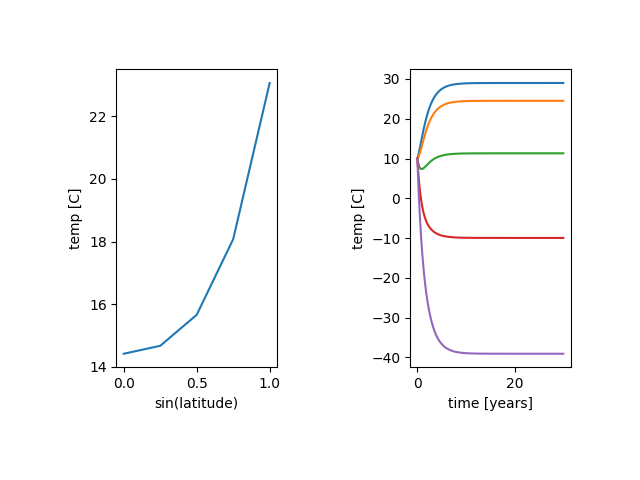
\includegraphics{n2e2.png}
\caption{$n = 2^2$}
\end{figure}

\begin{figure}
\centering
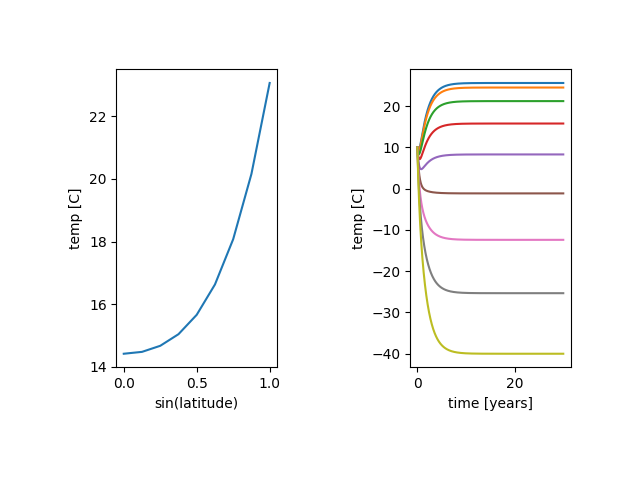
\includegraphics{n2e3.png}
\caption{$n = 2^3$}
\end{figure}

\begin{figure}
\centering
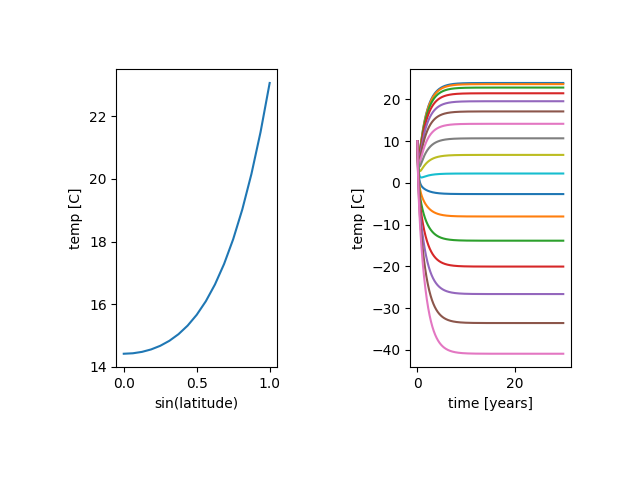
\includegraphics{n2e4.png}
\caption{$n = 2^4$}
\end{figure}


\begin{figure}
\centering
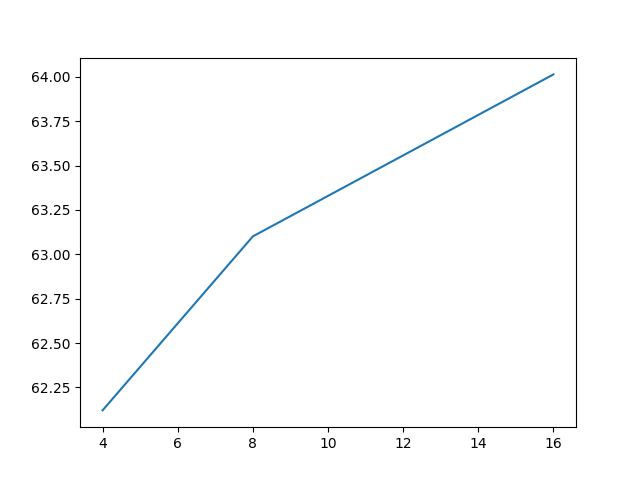
\includegraphics{nvserror.png}
\end{figure}




% Time / space efficiency of different t steps?

% TODO: See Budyko69, North et al 81 to see how these are parametrized. Also [2].
% asphalt ~ 
% open ocean ~ .1, see plots in [3]
% ocean ICE ~ 
% snow ~ 
% aluminum ~ higher than snow?




% DEFINITIONS

%\begin{defn}
%	Solar irradiance is the power per unit area, measured in $[W/m^2] = L^2 M T^{-3}$.
%	Power measured in Energy per unit time, energy supplied by the electro-magnetic
%	radiation from the sun.
%\end{defn}
%
%\begin{defn}
%	Incoming short-wave radiation from the sun is defined to be radiant energy with
%	wavelengths in the visible, near-ultraviolet and near-infrared spectra. This
%	gives us the wavelengths on the order of single micrometers.
%\end{defn}

% Q: To what degree does 02, water vapor, C02 as solar irradiance sinks in the
%		infrared regime (and O3 on the other end of the spectrum, in the ultraviolet
%		regime) indicate departure of reality from "earth as black body". How to 
%		quantify?

\end{document}

%% REFERENCES:
%	[1] https://www.e-education.psu.edu/meteo300/node/683
%	[2] Sea-ice albedo climate feedback mechanism - Curry, Schramm, Ebert 1994
%	[3] A parametrization of ocean surface albedo - Jin, Charlock, Smith, Rutledge 2004
%	[4] Finite difference methods - Leveque
%	[5] Budyko 1969





